\documentclass{amsart}
\usepackage{amsmath, amsfonts, amssymb}
\usepackage{tikz-cd}
\usepackage{bm}
\usepackage[boxruled, noend]{algorithm2e}
\usepackage{graphicx}

% hyperref
\usepackage[bookmarks=true,
bookmarksnumbered=true, breaklinks=true,
pdfstartview=FitH, hyperfigures=true,
plainpages=false, naturalnames=true,
colorlinks=true, pagebackref=true,
pdfpagelabels]{hyperref}
\hypersetup{
	linktocpage,
	colorlinks,
	citecolor=blue,
	linkcolor=blue,
	urlcolor=blue}

% layout
\setlength{\textwidth}{\paperwidth}
\addtolength{\textwidth}{-1.5in}
\setlength{\textheight}{\paperheight}
\addtolength{\textheight}{-2in}
\calclayout

% update to MSC2020
\makeatletter
\@namedef{subjclassname@2020}{%
	\textup{2020} Mathematics Subject Classification}
\makeatother

\newcommand{\W}{\mathsf{W}}
\newcommand{\F}{\mathbb{F}}
\renewcommand{\S}{\mathrm{S}}
\renewcommand{\k}{\Bbbk}
\renewcommand{\th}{\mathrm{th}}
\DeclareMathOperator{\xor}{\triangle}
\DeclareMathOperator{\eval}{eval}
\DeclareMathOperator{\pos}{pos}
\newcommand{\bu}{{\bar{u}}}
\newcommand{\sm}{\smallsetminus}
\newcommand{\R}{\mathbb{R}}
\newcommand{\RP}{\mathbb{R}\mathrm{P}}
\newcommand{\suspension}{\Sigma}

\newcommand{\Z}{\mathbb{Z}}
\renewcommand{\P}{\mathrm{P}}
\newcommand{\D}{\mathrm{D}}
\newcommand{\chains}{C_\bullet}
\newcommand{\cochains}{C^\bullet}
\newcommand{\Hom}{\mathrm{Hom}}
\newcommand{\Mod}{\mathbf{Mod}_{\F}}
\newcommand{\cMod}{\mathbf{Mod}_{\F}^{\simplex}}
\newcommand{\Ch}{\mathbf{Ch}_{\F}}
\newcommand{\cCh}{\mathbf{Ch}_{\F}^{\simplex}}
\newcommand{\sSet}{\mathbf{sSet}}
\newcommand{\id}{\mathrm{id}}
\newcommand{\ind}{\mathrm{ind}}
\newcommand{\p}{\mathrm{p}}
\newcommand{\q}{\mathrm{q}}
\newcommand{\Sq}{\mathrm{Sq}}
\newcommand{\simplex}{\bm{\Delta}}

\DeclareMathOperator*{\displaytensor}{\otimes}

% environment
\newtheorem{theorem}{Theorem}
\newtheorem{proposition}[theorem]{Proposition}
\newtheorem{lemma}[theorem]{Lemma}
\newtheorem{corollary}[theorem]{Corollary}
\newtheorem{claim}[theorem]{Claim}
\theoremstyle{definition}
\newtheorem{definition}[theorem]{Definition}
\newtheorem{example}[theorem]{Example}
\newtheorem{remark}[theorem]{Remark}
\newenvironment{tab}{\list{}{\rightmargin 0pt}\item\relax}{\endlist}

% other
\newcommand{\anibal}[1]{\textcolor{blue}{\underline{Anibal}: #1}}
\renewcommand{\th}{^\mathrm{th}}

\begin{document}	
	\title{New formulas for the cup-$i$ products and fast computation of Steenrod squares}
	\author{Anibal M. Medina-Mardones}
	\address{Department of Mathematics, University of Notre Dame}
	\email{amedinam@nd.edu}
	
	\begin{abstract}
		We present new formulas for cup-$i$ products on the simplicial cochains of a space and use them to introduce a fast algorithm for the computation of Steenrod squares on simplicial cohomology.
	\end{abstract}
	
	\maketitle
	\tableofcontents	
	
\section{Introduction}

For effective computations involving topological spaces, discrete models are indispensable.
The category of simplicial complexes provides models not only for spaces but also, through the simplicial approximation theorem, for continuous maps between them.
We can obtain from these combinatorial models algebraic ones using the simplicial chains construction $\chains$.
In this algebraic representation, invariants of spaces such as their betti numbers can be readily computed through linear algebra alone.

In this article we focused on finer invariants of spaces enriching their mod 2 cohomology and going beyond betti numbers.
We are referring to the celebrated Steenrod squares
\begin{equation*}
Sq^k \colon H^\bullet(X; \F_2) \to H^\bullet(X; \F_2).
\end{equation*}
These operations can be thought of as arising from the broken $\S_2$-symmetry of the diagonal map
\begin{equation*}
\begin{tikzcd}[column sep=small, row sep=-3pt]
X \arrow[r] & X \times X \\
x \arrow[r, mapsto] & (x,x)
\end{tikzcd}
\end{equation*}
occurring during the passage from continuous objects to discrete/algebraic models.

For simplicial complexes, effective constructions of Steenrod squares have been known since their introduction in Steenrod's seminal 1947 paper \cite{steenrod47}.
They all rely on the construction of \textit{cup-$i$ coproducts}
\begin{equation*}
\Delta_i \colon \chains(X; \F_2)  \to \chains(X; \F_2)^{\otimes 2}\,,
\end{equation*}
i.e., natural linear maps satisfying
\begin{equation*}
(1 + T) \Delta_{i-1} = \partial \circ \Delta_i + \Delta_i \circ \partial
\end{equation*}
for every integer $i$, and such that $\Delta_0$ is a chain approximation to the diagonal of $X$.

We will also consider \textit{cup-$i$ products}
\begin{equation*}
\smallsmile_i \colon \cochains(X; \F_2)^{\otimes 2} \to \cochains(X; \F_2),
\end{equation*}
the maps on cochains induced by linear duality.

Several constructions of cup-$i$ coproducts have been given in the literature starting with Steenrod's original formulas.
These include those resulting from the approach of Real \cite{real1996computability} and Gonz\'alez-D\'iaz--Real \cite{gonzalez1999combinatorial, gonzalez2003computation, gonzalez2005hpt} based on the EZ-AW chain contraction, the operadic methods of McClure-Smith \cite{mcclure03cochain} and Berger-Fresse \cite{berger04combinatorial}, and the prop viewpoint of the author \cite{medina2020prop1, medina2018prop2}.
Although it has been shown that all of these define isomorphic cup-$i$ coproducts \cite{medina2018axiomatic}, each presents advantages on different tasks.
For the effective computation of Steenrod squares on simplicial complexes, an algorithm based on \cite{gonzalez1999combinatorial} was implemented in the open-source mathematics system \verb|SAGE| by John Palmieri \cite{sagemath}.

In this article we introduce a new description of Steenrod's cup-$i$ coproducts.
We are particularly interested in simplicial complexes, but we remark that our formulas apply to the more general context of simplicial sets, a categorical closure of simplicial complexes that includes, for example, the singular cochains of a topological space.

For simplicial complexes we use our formulas to introduce a new algorithm computing Steenrod square.
Additionally, we report a performance comparison between a \verb|Python| implementation of our algorithm and the one in \verb|SAGE|.

The speed gained with our algorithm is essential for the incorporation of Steenrod squares into persistence homology \cite{medina2018persistence}, a technique typically used in highly intensive data analysis tasks \cite{carlsson2008images, carlsson2013viral, lee2018nanoporous} and for which various softwares \cite{bauer2019ripser, gudhi, medina2020giottotda} exist.

On the theoretical side, our formulas can serve as a template for the definition of mod 2 cohomology operations in other contexts.
For example, Cantero-Mor\'an \cite{cantero2020khovanov} followed this approach to define Steenrod squares in Khovanov homology.

Other areas besides topology where cup-$i$ coproducts and their dual products have become important include: condensed matter physics, where they are used to describe action functionals of discrete topological field theories \cite{gaiotto2016spin, bhardwaj2017state, kapustin2017fermionic}, higher category theory, where they can be used to deduce the nerve of $\omega$-categories \cite{medina2020globular}, and convex geometry, where they are connected to projections of cyclic polytopes \cite{kapranov1991combinatorial}.
It is our hope that the new description of cup-$i$ products presented in this article can serve to facilitate new connections and to deepen those already established.

In \cref{s:preliminaries} we review the notions from equivariant homological algebra and simplicial topology needed to present, in \cref{s:squares}, a definition of Steenrod squares in terms of cup-$i$ products.
We introduce our new formulas in \cref{s:formulas}, and our algorithm for the computation of Steenrod squares in \cref{s:algorithm}; providing a proof-of-concept comparison using \verb|SAGE| in \cref{s:comparison}.
In \cref{s:proof}, the technical core of this article, we prove that our new formulas define cup-$i$ coproducts, and in \cref{s:outlook} we discuss finer invariants associated to Steenrod squares.
	
\subsection*{Acknowledgments} We would like to thank Dennis Sullivan, Kathryn Hess, Stephan Stolz, Mark Behrens, John Morgan, Greg Brumfiel, Federico Cantero-Mor\'an, Pedro Real, Roc\'io Gonzalez-D\'iaz, Tim Campion, Riley Levy, Umberto Lupo, Guillaume Tauzin, and Matteo Caorsi for stimulating conversations about this project.
	
\section{Preliminaries} \label{s:preliminaries}

In this section we review the basic notions used in this article and set up the conventions we follow.

\subsection{Chain complexes}

We assume familiarity with the notion of chain complex over a ring $\k$. We will use homological grading regarding any cohomologically graded complex $A$ as homologically graded via $A_n = A^{-n}$.

The \textit{tensor product} $C \otimes C^\prime$ of $C$ and $C^\prime$ is the chain complex whose degree-$n$ part is
\begin{equation*}
\left(C \otimes C^\prime\right)_n = \bigoplus_{i+j=n} C_i \otimes C^\prime_j,
\end{equation*}
where $C_i \otimes C^\prime_j$ is the tensor product of $\k$-modules, and whose boundary map is defined by
\begin{equation*}
\partial (v \otimes w) = \partial v \otimes w + (-1)^{|v|} v \otimes \partial w.
\end{equation*}

The \textit{hom complex} $\Hom(C, C^\prime)$ is the chain complex whose degree-$n$ part is the subset of linear maps between them that increase degree by $n$, i.e.,
\begin{equation*}
\Hom(C, C^\prime)_n = \{f \mid f(C_k) \subseteq C^\prime_{k+n}\},
\end{equation*}
and boundary map defined by
\begin{equation*}
\partial f = \partial_{C^\prime} \circ f - (-1)^{n} f \circ \partial_C.
\end{equation*} 
Notice that a chain map is the same as a $0$-cycle in this complex, and that two chain maps are chain homotopy equivalent if and only if they are homologous cycles. We extend this terminology and say that two maps $f, g \in \Hom(C, C^\prime)$ are \textit{homotopic} if their difference is nullhomologous, referring to a map $h \in \Hom(C, C^\prime)$ such that $\partial h = f - g$ as a \textit{homotopy} between them.

Regarding $\k$ as a chain complex concentrated in degree $0$, the \textit{linear dual} of a chain complex $C$ is the chain complex $\Hom(C, \k)$.
We refer to the contravariant functor $\Hom(-, \k)$ as \textit{linear duality}.

For any three chain complexes, there is a natural isomorphism of chain complexes
\begin{equation} \label{e:adjunction isomorphism}
\Hom(C \otimes C^\prime, C^{\prime\prime}) \cong
\Hom(C, \Hom(C^\prime, C^{\prime\prime}))
\end{equation}
referred to as the \textit{adjunction isomorphism}.

\subsection{Group actions}

Symmetries on chain complexes play an important role on this work.
Let $G$ be a finite group.
We will later focus solely on the symmetric group $\S_2$.
We denote by $\k[G]$ the group ring of $G$, i.e., the free $\k$-module generated by $G$ together with the ring product defined by linearly extending the product of $G$.
We refer to a chain complex of left $\k[G]$-modules as a chain complex with a $G$-\textit{action} and to $\k[G]$-linear maps as $G$-\textit{equivariant}.

Given a chain complex $C$ with a $G$-action we naturally associate the following two chain complexes.
The subcomplex of \textit{invariant chains} of $C$, denoted $C^G$, contains all elements $c \in C$ satisfying $g \cdot c = c$ for every $g \in G$.
The quotient complex of \textit{coinvariant chains} of $C$, denoted $C_G$, is the chain complex obtained by identifying elements $c, c^\prime \in C$ if there exists $g \in G$ such that $c^\prime = g \cdot c$.

Let $C$ and $C^\prime$ be chain complexes and assume $C$ has a $G$-action.
The chain complex $\Hom(C, C^\prime)$ has a $G$-action induced from $(g \cdot f)(c) = f^{-1}(g^{-1} \cdot c)$ and there is an isomorphism
\begin{equation} \label{e:invariant hom iso hom coinvariants}
\Hom(C, C^\prime)^G \cong \Hom(C_G, C^\prime).
\end{equation}

\subsection{Simplicial topology}

Simplicial complexes are used to combinatorially encode the topology of spaces.
An \textit{abstract and ordered simplicial complex}, or a \textit{simplicial complex} for short, is a pair $(V, X)$ with $V$ a poset and $X$ a set of subsets of $V$ such that: 
\begin{enumerate}
	\item The restriction of the partial order of $V$ to any element in $X$ defines a total order on it.
	\item For every $v$ in $V$, the singleton $\{v\}$ is in $X$.
	\item If $x$ is in $X$ and $y$ is a subset of $x$, then $y$ is in $X$.
\end{enumerate}
We abuse notation and denote the pair $(V, X)$ simply by $X$ referring to $V$ as its poset of vertices.

The elements of $X$ are called \textit{simplices} and the \textit{dimension} of a simplex $x$ is defined by subtracting $1$ from the number of vertices it contains.
Simplices of dimension $n$ are called $n$-simplices and are denoted by their order set of vertices $[v_0, \dots, v_n]$.
The collection of $n$-simplices of $X$ is denoted $X_n$.
There are natural maps $d_i^n \colon X_n \to X_{n-1}$ for $i \in \{0, \dots, n\}$ defined by
\begin{equation*}
d_i^n([v_0, \dots, v_n]) = [v_0, \dots, \widehat{v}_i, \dots, v_n]
\end{equation*}
and referred to as the $i^{\th}$ face map in dimension $n$.
These satisfy the \textit{simplicial relation}:
\begin{equation} \label{e:simplicial relation}
d_i^{n-1} d^n_j = d_{j-1}^{n-1} d_i^n
\end{equation}
for any $0 \leq i < j \leq n$.
We will omit the superscripts of these maps when no confusion arises from doing so.

A \textit{simplicial map} $X \to X^\prime$ is a poset morphisms between their vertices $f \colon V \to V^\prime$ sending simplices to simplices, i.e., satisfying that if $[v_0, \dots, v_n] \in X$ then $[f(v_0), \dots, f(v_n)] \in X^\prime$.

Let $X$ be simplicial complex.
The degree-$n$ part of the chain complex of \textit{chains} of $X$, which we denote $\chains(X; \k)$, is defined by
\begin{equation*}
C_n(X; \k) = \k \big\{ X_n \big\},
\end{equation*}
i.e., the $\k$-module freely generated by the $n$-dimensional simplices of $X$.
The boundary map is defined on basis elements by
\begin{equation*}
\begin{tikzcd}[column sep=normal, row sep=tiny,row sep = 0ex
,/tikz/column 1/.append style={anchor=base east}
,/tikz/column 2/.append style={anchor=base west}
]
C_n(X; \k) \arrow[r, "\partial_n"] & C_{n-1}(X; \k) \\
x\ \arrow[r, |->] & \sum_{i=0}^{n} (-1)^i d_i (x).
\end{tikzcd}
\end{equation*}

Given a simplicial map $f \colon X \to X^\prime$, the \textit{induced map} $f_\bullet \colon \chains(X; \k) \to \chains(X^\prime; \k)$ is the chain map defined on basis elements by $f_\bullet([v_0, \dots, v_n]) = [f(v_0), \dots, f(v_n)]$ if $i \neq j$ implies $ f(v_i) \neq f(v_j)$ and it is $0$ otherwise.

We referred to
\begin{equation*}
\cochains(X; \k) = \Hom(\chains(X; \k), \k)
\end{equation*}
as the \textit{cochains} of $X$ and to the dual $\delta^{n}$ of $\partial_{-n}$ as the $n\th$ coboundary map.
Furthermore, we denote the linear dual of the map $f_\bullet$ induced by a simplicial map $f$ by $f^\bullet$.
We remark that $C_n(X; \k) = 0$ for $n < 0$ and $C^n(X;\k) = 0$ for $n > 0$.

The \textit{homology} $H_\bullet(X; \k)$ and \textit{cohomology} $H^\bullet(X; \k)$ of $X$ are defined by applying the kernel-mod-image construction to $\chains(X; \k)$ and $\cochains(X; \k)$ respectively.
More specifically, a (co)homology class in degree $n$ is an equivalence class of elements in the kernel of the $n\th$ (co)boundary map, referred to as  $n\th$\textit{(co)cycles}, where two are regarded as equivalent if their difference is in the image of the $(n+1)\th$ (co)boundary map.

When $X$ and $\k$ are clear from the context we omit them from the notation.
	
\section{Cup-$i$ products and Steenrod squares} \label{s:squares}

Let $\F_2$ be the field with two elements and $\S_2$ the group with only one non-identity element $T$.
In this section we define for any simplicial complexes $X$ and every integer $k$ the Steenrod $k^{\mathrm{th}}$ square
\begin{equation*}
Sq^k \colon H^\bullet(X; \F_2) \to H^{\bullet}(X; \F_2)
\end{equation*}
using an arbitrary cup-$i$ construction.

Consider the chain complex
\begin{equation*}
\begin{tikzcd}[column sep=normal]
& W =  \F_2[\S_2]\{e_0\} & \arrow[l, "1+T"'] \F_2[\S_2]\{e_1\} & \arrow[l, "1+T"']
\F_2[\S_2]\{e_2\} & \arrow[l, "1+T"'] \cdots
\end{tikzcd}
\end{equation*}
with its natural $\S_2$-action.

For any simplicial complex $X$, consider an $\S_2$-equivariant chain map
\begin{equation} \label{e:steenrod diagonal}
\Delta_X \colon W \otimes \chains(X; \F_2) \to \chains(X; \F_2)^{\otimes 2}
\end{equation}
where the $\S_2$-action in the domain is concentrated in $W$ and in the target is the transposition of factors $T(a \otimes b) = b \otimes a$.
We say that this collection of maps is natural if for any simplicial map $f \colon X \to Y$ we have $\Delta_Y \circ f_\bullet = f_\bullet^{\otimes 2} \circ \Delta_X$, and we say that is \textit{cup-$i$ construction} if it is natural and the image of a $0$-simplex is not 0.

A cup-$i$ construction is determined by a collection $\{\Delta_i\}_{i \in \Z}$ of natural linear maps $\chains \to \chains^{\otimes 2}$ satisfying $\Delta_0 \big([v_0]\big) \neq 0$ for any vertex $v_0$ and
\begin{equation} \label{e:boundary of cup-i}
(1 + T) \Delta_{i-1} = \partial \circ \Delta_i + \Delta_i \circ \partial
\end{equation}
for any $i \in \Z$.
The correspondence is given by $\Delta_i = \Delta(e_i \otimes -)$, and we refer to the map $\Delta_i$ as the \textit{cup-$i$ coproduct} of the cup-$i$ construction, and to the linear dual $\smallsmile_i$ of $\Delta_i$ as its \textit{cup-$i$ product}.

Let us consider a cup-$i$ construction $W \otimes C_\bullet \to C_\bullet^{\otimes 2}$.
Using the linear duality functor and passing to fix points gives a chain map
\begin{equation*}
\begin{tikzcd}
\Hom\left(C_\bullet \otimes C_\bullet, \F_2 \right)^{\mathrm S_2} \arrow[r] &
\Hom\left(W(2) \otimes C_\bullet, \F_2 \right)^{\mathrm S_2},
\end{tikzcd}
\end{equation*}
which we can complete, using the adjunction isomorphisms of \cref{s:preliminaries}, to a commutative diagram
\begin{equation*}
\begin{tikzcd}
\Hom\left(C_\bullet \otimes C_\bullet, \F_2 \right)^{\mathrm S_2} \arrow[r] &
\Hom\left(W(2) \otimes C_\bullet, \F_2 \right)^{\mathrm S_2} \arrow[d] \\
\left(C^\bullet \otimes C^\bullet\right)^{\mathrm S_2} \arrow[u]&
\Hom\left(W(2)_{\mathrm S_2} \otimes C_\bullet, \F_2 \right) \arrow[d] \\
C^\bullet \arrow[u, "doubleing"] \arrow[r, dashed]&
\Hom\left(W(2)_{\mathrm S_2}, C^\bullet\right),
\end{tikzcd}
\end{equation*}
where the choice of coefficients ensures the \textit{doubleing map} $\alpha \mapsto \alpha \otimes \alpha$ is linear.
Using the adjunction isomorphism \eqref{e:adjunction isomorphism}, the dashed arrow defines a linear map
\begin{equation} \label{e:Steenrod squares parameterized}
\begin{tikzcd}[row sep=0pt, column sep = tiny]
C^\bullet \otimes W(2)_{\mathrm S_2} \arrow[r] &[-10pt] C^\bullet \\
\alpha \otimes e_i \arrow[r, |->] & (\alpha \otimes \alpha)\Delta_i(-)
\end{tikzcd}
\end{equation}
descending to mod $2$ cohomology.
The \textit{Steenrod squares}, whose importance in homotopy theory is hard to overstate, are defined by reindexing this map.
Explicitly,
\begin{equation*}
\begin{tikzcd}[row sep=0pt, column sep=tiny]
Sq^k \colon H^{-n} \arrow[r] & H^{-n-k} \\
\phantom{Sq^k \colon}{[\alpha]} \arrow[r, |->] & {\left[(\alpha \otimes \alpha)\Delta_{n-k}(-) \right]}.
\end{tikzcd}
\end{equation*}

\begin{remark}
	Although in this article we do not use the algebra structure on the mod 2 cohomology of spaces, we remark that the cup-$0$ product of a cup-$i$ construction represents the product of this algebra.
	Explicitly, if $[\alpha], [\beta] \in H^\bullet$ then $[\alpha][\beta] = [\alpha \smallsmile_0 \beta]$, in particular, if $[\alpha]$ is of degree $-k$ then $\Sq^k\big([\alpha]\big) = [\alpha] [\alpha]$, which motivates the name of these operations.
\end{remark}

\begin{remark}
	For the reader familiar with group homology, we remark that Steenrod squares are parameterized by classes on the mod $2$ homology of $\mathrm S_2$.
	Steenrod later used this group homology viewpoint to define non-constructively for any prime $p$ operations on the mod $p$ cohomology of spaces \cite{steenrod1962cohomology}.
	Analogues of the $\Delta_i$ maps for odd primes that define these operations constructively were introduced in \cite{medina2020odd} and implemented in \cite{medina2021computer}.
\end{remark}
	
\section{New formulas} \label{s:formulas}

In this section we introduce our new description of cup-$i$ coproducts.
We define them for simplicial complexes although there is no obstruction interpreting these formulas as defining cup-$i$ coproducts on simplicial sets \cite{friedman2012simplicial}, a more general notion.

Let $X$ be a simplicial complex and $x \in X_n$.
For a set
\begin{equation*}
U = \{u_1 < \dots < u_r\} \subseteq \{0, \dots, n\}
\end{equation*}
we use the notation $d_U(x) = d_{u_1} \ldots\, d_{u_r}(x)$, with $d_{\emptyset}(x) = x$.

\begin{definition} \label{d:cup-i coproducts}	
	For any simplicial complex $X$ and an integer $i$, the \textit{cup-$i$ coproduct}
	\begin{equation*}
	\Delta_i : C_\bullet(X; \F_2) \to C(X; \F_2)^{\otimes 2}_\bullet
	\end{equation*}
	is the linear map defined on a basis element $x \in X_n$ to be $0$ if $i \not\in \{0, \dots, n\}$ and otherwise by
	\begin{equation} \label{equation: simplicial cup-i coproducts}
	\Delta_i(x) = \sum d_{U^0}(x) \otimes d_{U^1}(x),
	\end{equation}
	where the sum is taken over all sets $U = \{u_1 < \cdots < u_{n-i}\}$ with $u_j \in \{0, \dots, n\}$ and where
	\begin{equation*}
	U^0 = \{u_j \in U\ |\ u_j \equiv j \text{ mod } 2\}, \qquad
	U^1 = \{u_j \in U\ |\ u_j \not\equiv j \text{ mod } 2\}.
	\end{equation*}
\end{definition}

\begin{example}
	For any $x \in X_n$ and $i = 0$ the formula above reduces to
	\begin{equation*}
	\Delta_0(x) = \sum_{i=0}^n d_{i+1} \cdots d_{n}(x) \otimes d_{0} \cdots d_{i-1}(x),
	\end{equation*}
	a map known as Alexander-Whitney diagonal and widely used to define the algebra structure on cohomology.
\end{example}

\begin{example}
	For any basis element $x \in X_n$ we have
	\begin{equation*}
	\Delta_n(x) = x \otimes x,
	\end{equation*}
	implying that $Sq^0$ is the identity in cohomology.
\end{example}

\begin{theorem}
	The maps introduced in Definition~\ref{d:cup-i coproducts} define a cup-$i$ construction.
\end{theorem}

Since by the previous examples the maps are not identically zero, we need to check they are natural with respect to simplicial maps and that they satisfy \eqref{e:boundary of cup-i}.
We state these claims as a pair of lemmas.

\begin{lemma}
	If $f$ is a simplicial map, then, for every $i \in \Z$,
	\begin{equation*}
	\Delta_i \circ f_\bullet = (f_\bullet \otimes f_\bullet) \circ \Delta_i.
	\end{equation*}
\end{lemma}

\begin{proof}
	Consider a basis element $x = [v_0, \dots, v_n]$ and first assume that $f_\bullet(x)$ is not $0$.
	Then, for any subset $U$ of $\{0, \dots, n\}$ the image of $d_U(x)$ is not $0$ as well and we have
	\begin{align*}
	\Delta_i \circ f_\bullet(x) =\ &
	\Delta_i \big([f(v_0), \dots, f(v_n)]\big) \\ =\ &
	\sum d_{U^0} \big([f(v_0), \dots, f(v_n)]\big) \otimes d_{U^1} \big([f(v_0), \dots, f(v_n)]\big) \\ =\ &
	(f_\bullet \otimes f_\bullet) \sum d_{U^0} \big([v_0, \dots, v_n]\big) \otimes d_{U^1} \big([v_0, \dots, v_n]\big) \\ =\ &
	(f_\bullet \otimes f_\bullet) \circ \Delta(x).
	\end{align*}
	If $f_\bullet(x) = 0$ then there exists consecutive elements $v_j$ and $v_{j+1}$ with $f(v_j) = f(v_{j+1})$.
	To prove that $(f_\bullet \otimes f_\bullet) \circ \Delta(x) = 0$ it suffices to show that for any $U \in \P_{n-i}(n)$ either the simplex $f \big(d_{U^0}(x) \big)$ or $f \big( d_{U^1}(x) \big)$ contains both $v_j$ and $v_{j+1}$.
	If $U$ does not contain both $j$ and $j+1$ this is immediate.
	If it does we have that	$j, j+1 \in U^0$ or $j, j+1 \in U^1$ since they are consecutive so $\ind_U(i) = \ind_U(i+1)$.
\end{proof}

\begin{lemma} \label{l:main}
	For any integer $i$,
	\begin{equation} \label{eq: cup-i coproducts boundary relation}
	\partial \circ \Delta_{i} + \Delta_{i+1} \circ \partial = (1 +T ) \Delta_{i-1}.
	\end{equation}
\end{lemma}

We devote Section~\ref{s:proof} to the proof of this theorem.
	
\section{New algorithm for Steenrod squares} \label{s:algorithm}

%Throughout this section we use $\Delta_i$ to denote the $i\th$ map introduced in \cref{d:cup-i coproducts}.

For a finite simplicial complex $X$ we now present an algorithm effectively constructing a cocycle representing $Sq^k([\alpha])$ given a cocycle $\alpha$.

Let $-n$ be the degree of $\alpha$ and let $A = \{a_1, \dots, a_m\} \subseteq X_n$ with $\alpha = \alpha_1 + \cdots + \alpha_m$ and
\begin{equation*}
\alpha_i(a_j) = \begin{cases}
1 & i=j, \\ 0 & i\neq j.
\end{cases}
\end{equation*}
If $k < 0$ or $k > n$, we have by definition that $Sq^k([\alpha]) = 0$ and we can take $0$ as its representative.
If $k = 0$, \cref{ex:Sq0 is the identity} shows that $Sq^0([\alpha]) = [\alpha]$ so we can take $\alpha$ as its representative.
For $k \in \{1, \dots, n\}$ we will construct a set $B \subseteq X_{n+k}$ such that if $\beta = (\alpha \otimes \alpha)\Delta_{n-k}(-)$, where $\Delta_{n-k}(-)$ is presented in \cref{d:cup-i coproducts}, we have
\begin{equation} \label{e:correctness}
\beta(x) =
\begin{cases}
1 & x \in B, \\
0 & x \not\in B,
\end{cases}
\end{equation}
for any basis element $x \in X_{n+k}$.

Consider \cref{a:algorithm} presented in \cref{f:algorithm} and let $B \subseteq X_{n+k}$ be its output when the input is $A$.

\begin{figure}
	%!TEX root = ../fast_sq.tex

\begin{algorithm} [H]
	\KwIn{$A = \{a_1, \dots, a_m\} \subseteq X_n$}
	$B = \emptyset$\\
	\ForAll{$a_i\ \mathrm{and}\ a_j\ \mathrm{with}\ i < j$}
	{
		$a_{ij} = a_i \cup a_j$\\
		\If{$a_{ij} \in X_{n+k}$}
		{
			$\overline{a}_i = a_i \setminus a_j$\ ;\ \
			$\overline{a}_j = a_j \setminus a_i$\ ;\ \
			$\overline{a}_{ij} = \overline{a}_i \cup \overline{a}_j$ \\
			$\ind \colon \overline{a}_{ij} \to \{0,1\}$ \\
			\ForAll {$v \in \overline{a}_{ij}$}
			{
				$p = \mathrm{position\ of\ } v \mathrm{\ in\ } a_{ij}$\ ;\ \
				$\overline{p} = \mathrm{position\ of\ } v \mathrm{\ in\ } \overline{a}_{ij}$\\
				$\ind(v) = {p}\, +\, \overline{p}\ \ \mathrm{residue\ mod}\ 2$
			}
			\If{\hspace*{3pt}$\ind(\overline{a}_i) \xor \ind(\overline{a}_j)$ = $\{0,1\}$}
			{$B = B \xor \, \{a_{ij}\}$}
		}
	}
	\KwOut{$B \subseteq X_{n+k}$}
	\caption{$SQ^k_n$}
	\label{a:algorithm}
\end{algorithm}
	\caption{Algorithm producing for a simplicial complex $X$, non-negative integer $n$, integer $k$ between $1$ and $n$, and cocycle $\alpha$ presented as a set $A \subseteq X_n$, a cocycle representing $Sq^k([\alpha])$ returned as a set $B \subseteq X_{n+k}$.
		We use the notation $S \xor S^\prime = S \cup S^\prime \setminus (S \cap S^\prime)$.}
	\label{f:algorithm}
\end{figure}

Before verifying \eqref{e:correctness}, let us record a property satisfied by our cup-$i$ construction that can be thought of as a form of ``freeness".

\begin{lemma} \label{l:freeness}
	Let $\gamma_1 + \cdots + \gamma_m$ be the basis representation of a cochain in $C^{-n}(X; \Ftwo)$.
	For integers $k$ and $i, j \in \{1, \dots, m\}$ with $i \neq j$, and any $x \in X_{n+k}$:
	\begin{enumerate}
		\item if $k \neq 0$, then $(\gamma_i \otimes \gamma_i)\Delta_{n-k}(x) = 0$,
		\item if $(\gamma_i \otimes \gamma_j)\Delta_{n-k}(x) \neq 0$, then $(\gamma_j \otimes \gamma_i)\Delta_{n-k}(x) = 0$,
	\end{enumerate}
	where $\Delta_{n-k}$ is the $(n-k)\th$ map introduced in \cref{d:cup-i coproducts}.
\end{lemma}

\begin{proof}
	Recall that
	\begin{equation*}
	\Delta_{n-k}(x) \ = \! \sum_{\substack{U \subseteq \{0, \dots, n\} \\ \vert U \vert = k}}
	d_{U^0}(x) \otimes d_{U^1}(x).
	\end{equation*}

	If $(\gamma_i \otimes \gamma_j)\Delta_{n-k}(x) \neq 0$, then there exists a non-empty $U$ in the sum with $U^0 = U^1$, which is impossible since $U^0 \cap U^1 = \emptyset$.

	If $(\gamma_i \otimes \gamma_j)\Delta_{n-k}(x) \neq 0$ and $(\gamma_j \otimes \gamma_i)\Delta_{n-k}(x) \neq 0$, then there are distinct subsets $V$ and $W$ in the sum such that $V^0 = W^1$ and $W^0 = V^1$, which is impossible since $V = V^0 \cup V^1 = W^0 \cup W^1 = W$.
\end{proof}

Let us now return to the correctness of the algorithm.
For any $x \in X_{n+k}$ the value of $\beta$ evaluated on the chain represented by $x$ is given by
\begin{align*}
\beta(x) & =
(\alpha \otimes \alpha) \Delta_{n-k}(x) \\ & =
(\alpha_1 + \cdots + \alpha_m)^{\otimes 2} \Delta_{n-k}(x) \\ & =
\Big(\sum_{i \neq j} \alpha_i \otimes \alpha_j + \sum_{i} \alpha_i \otimes \alpha_i \Big)
\Delta_{n-k}(x) \\ & =
\Big(\sum_{i \neq j} \alpha_i \otimes \alpha_j\Big)
\Delta_{n-k}(x).
\end{align*}
By \cref{l:freeness}, at most one of the terms $\alpha_i \otimes \alpha_j$ or $\alpha_j \otimes \alpha_i$ evaluates to $1$ on $\Delta_{n-k}(x)$, so to determine the value of $\beta(x)$ we need to count mod 2 the number of subsets $\{i,j\} \subseteq \{1,\dots, m\}$ such that $\{a_i, a_j\} = \{d_{U^0}(x), d_{U^1}(x)\}$ for some $U \subseteq \{0, \dots, n\}$ of cardinality $k$.
This condition on the pair $\{a_i, a_j\}$ implies in particular that $a_i \cup a_j = x$ since $d_{U^0}(x) \cup d_{U^1}(x) = x$.

Let us formalize these observations.
Let $\widetilde{A}$ be the set of all two-element subsets $\{a_i, a_j\} \subseteq A$ with $a_i \cup a_j \in X_{n+k}$.
There is a natural map $\pi \colon \widetilde{A} \to X_{n+k}$ sending $\{a_i, a_j\}$ to $a_i \cup a_j$.
Let $\eval \colon A \to \Ftwo$ be the map sending $\{a_i, a_j\}$ to $1$ if there exist $U \subseteq \{0,\dots,n\}$ of cardinality $k$ such that $\{a_i, a_j\} = \{d_{U^0}(x), d_{U^1}(x)\}$ and let $\eval(\{a_i, a_j\}) = 0$ otherwise.
Notice that if such $U$ exists then it is unique.
With this notation we have
\begin{equation*}
\beta(x) \ = \! \sum_{\{a_i, a_j\} \in \pi^{-1}(x)} \! \eval(\{a_i, a_j\}).
\end{equation*}
We will give a computational characterization of $\eval(\{a_i, a_j\}) = 1$ after introducing some more notation.

Given a finite totally ordered set $S$, the \textit{position function} $\pos_S \colon S \to \Z$ sends an element $s \in S$ to the cardinality of $\{s^\prime \in S \mid s^\prime \leq s\}$.
Denote
\begin{equation*}
\overline{a}_{i} = a_i \setminus a_j, \qquad
\overline{a}_{i} = a_i \setminus a_j, \qquad
\overline{a}_{ij} = \overline{a}_i \cup \overline{a}_j.
\end{equation*}
Given $\{a_i, a_j\} \in \pi^{-1}(x)$, there exists $U$ with $\{a_i, a_j\} = \{d_{U^0}(x),\, d_{U^1}(x)\}$
if and only if $U = \pos_{x}(\overline{a}_{ij})$ and
\begin{equation} \label{e:pos's equal U's}
\big\{\pos_{x}(\overline{a}_i),\, \pos_{x}(\overline{a}_j)\big\} = \{U^0, U^1\}.
\end{equation}
Recall that $U^0$ (resp. $U^1$) is the subset of $U \subseteq \{0, \dots, n+k\}$ with elements satisfying that their position in $U$ plus its position in $\{0, \dots, n+k\}$ is $0$ mod 2 (resp. $1$ mod 2).
Therefore, \eqref{e:pos's equal U's} is equivalent to the function $\ind \colon \pos_x(\overline{a}_{ij}) \to \Ftwo$ defined by
\begin{equation*}
\ind(v) = \pos_{x}(v) + \pos_{\overline{a}_{ij}}(v) \text{ mod }2
\end{equation*}
being constant on both $\overline{a}_i$ and $\overline{a}_j$ with different values, i.e.,
\begin{equation*}
\ind(\overline{a}_i) \xor \ind(\overline{a}_j) = \{0,1\}.
\end{equation*}

Therefore, for any $x \in X_{n+k}$ we have $\beta(x) = 1$ if and only if the set of pairs $\{a_i, a_j\}$ in $\pi^{-1}(x)$ with $\eval(\{a_i, a_j\}) = 1$ is odd; which is equivalent to the condition $x \in B$.
	
\section{Performance comparison} \label{s:comparison}

In this section we present a proof-of-concept comparison between the existing method for the computation of Steenrod squares on simplicial complexes, based on Gonz\'alez-D\'iaz--Real's approach \cite[Corollary 3.2]{gonzalez1999combinatorial}, and the one introduced here.
We used a \verb|Python| implementation of our algorithm and the open source computer algebra system \verb|SAGE v9.3.rc3| \cite{sagemath} which includes an implementation of the existing method written by John Palmieri.

Given a topological space $X$ the \textit{suspension} of $X$ is the topological space $\suspension X$ obtained from $X \times [0,1]$ by collapsing $X \times \{0\}$ and $X \times \{1\}$ to points.
Suspension is a natural construction and, for each integer $i \neq 0$, there is an isomorphism $H^i(X) \cong H^{i+1}(\suspension X)$, which can be extended to $i = 0$ by considering reduced cohomology.
A crucial fact about Steenrod squares is that for reduced cohomology with mod 2 coefficients, all operations commuting with the suspension isomorphism are generated by the Steenrod squares.

The real projective plane $\RP^2$, obtained by identifying antipodal points in a sphere, is the simplest space with a non-trivial Steenrod square.
Its reduced mod 2 cohomology has a single basis element $x_i \in \widetilde{H}^i(\RP^2; \F_2)$ for $i \in \{1, 2\}$ and satisfies $Sq^1(x_1) = x_2$.
Therefore, its $i\th$ suspension $\suspension^i \RP^2$ has a non-trivial operation given by $Sq^1(\suspension^i x_1) = \suspension^i x_2$.

We now describe the pipeline we followed for the comparison.
In \verb|SAGE| we produced a simplicial complex model of $\suspension^i \RP^2$ for each $i \in \{0, \dots, 10\}$ using the methods \verb|RealProjectiveSpace(2)| and \verb|suspension(i)|.
We used the \verb|cohomology_ring(GF(2))| method on this model and on its output the method \verb|basis()| to obtain a model for the element $\suspension^i x_1$.
Finally we applied the method \verb|Sq(k)| to it with $k=1$ and record the execution time of this last step.
We implemented in \verb|Python| an alternative for the method \verb|Sq(k)| based on \cref{a:algorithm} and modified the above pipeline accordingly.
We recorded the average execution time of these implementations for each $\suspension^i \RP^2$ over $\lfloor 10000/2^i \rfloor$ runs for each $i \in \{0, \dots, 10\}$.
The results of this pipeline are presented in \cref{f:comparison}.
We notice that the execution time of the implementation based on our algorithm remains constant whereas the one in \verb|SAGE| grows exponentially.

\begin{figure}
	\includegraphics[width=0.9\textwidth]{comp_sus_rp2.pdf}
	\caption{Average execution time in \texttt{SAGE} of two methods computing Steenrod squares. In orange the one proposed in this article and in blue the one included in \texttt{SAGE v9.3.rc3}. More specifically, for each $i \in \{0, \dots, 10\}$ we timed the computation of the non-trivial Steenrod square in the cohomology of the $i\th$ suspension of the real projective plane, averaged over a number of runs equal to the integral part of $\frac{10000}{2^i}$.}
	\label{f:comparison}
\end{figure}
	
\section{Proof of Theorem~\ref{t:main}} \label{s:proof}

To aid readability of the relatively long proof of this theorem we split it into four lemmas.
We start with some notation.

\begin{definition}
	Let $\P_q(n)$ be the set of all sets $U = \{u_1 < \cdots < u_{n-i}\}$ with $u_j \in \{0, \dots, n\}$.
	For any $U \in \P_q(n)$, let $\overline{U} \in \P_{n+1-q}(n)$ contain the elements of $\{0, \dots, n\}$ not in $U$. For $x \in \overline{U}$, define $x.U \in \P_{q+1}(n)$ to contain $x$ and the elements in $U$.
	For $x \in U$, define $U \setminus x \in \P_{q-1}(n)$ to contain the elements in $U$ different from $x$.
\end{definition}

Recall that for any $U = \{u_1 < \cdots < u_q\} \in \P_q(n)$ we write $d_U$ for $d_{u_1}^{n-q+1} \cdots \,d_{u_q}^n$ and avoid writing the superscripts when they do not contribute to expositional clarity.
With this notation we have for any $x \in X_n$
\begin{equation*}
\Delta_{n-q}(x)\ =\! \sum_{U \in \P_q(n)} d_{U^+}(x) \otimes d_{U^-}(x).
\end{equation*}

\begin{lemma} \label{l:partial dU = dxU}
	For any $x \in X_n$ and $U \in \P_{q}(n)$
	\begin{equation} \label{lemma1: existence: eq1}
	\partial \circ d_U(x) = \sum_{\bar{u} \in \overline{U}} d_{\bar{u}.U}(x).
	\end{equation}
\end{lemma}

\begin{proof}
	Let $U = \{u_1 < \cdots < u_q\}$. Using the simplicial relation \eqref{e:simplicial relation} we have
	\begin{equation*}
	\partial \circ d_U(x) = 
	\sum_{i=0}^{n-q} d_i\, d_{u_1} \cdots\, d_{u_q}(x) = 
	\sum_{\bar{u} \in \overline{U}} d_{u_1} \cdots\, d_{\bar{u}} \cdots\, d_{u_q}(x) =
	\sum_{\bar{u} \in \overline{U}} d_{\bar{u}.U}(x)
	\end{equation*}
	as claimed.
\end{proof}

\anibal{Check the $q=0$ case below.}

\begin{lemma} \label{l:pigeon hole}
	For any $x \in X_n$ and $q \in \{0, \dots, n\}$
	\begin{equation} \label{e:pigeon hole 1}
	\Delta_{n-q-1} \circ \partial (x)\ =\! 
	\sum_{U \in \P_q(n)} \left( 
	\sum_{u \in U^-} d_{u.U^+}(x) \tensor d_{U^-}(x) + 
	\sum_{u \in U^+} d_{U^+}(x) \tensor d_{u.U^-}(x) \right).
	\end{equation}
\end{lemma}

\begin{proof}
	Let
	\begin{align*}
	& S_1 = \big\{ (u, V)\ |\ V \in \P_{q-1}(n-1) \text{ and } u \in \{0,\dots,n\} \big\}, \\
	& S_2 = \big\{ (w, W)\ |\ W \in \P_{q}(n) \text{ and } w \in W \big\}
	\end{align*}
	and notice that identity \eqref{e:pigeon hole 1} is equivalent to the following identity:
	\begin{equation} \label{e:pigeon hole 2}
	\sum_{(u, V) \in S_1} d_{V^+}d_u \tensor d_{V^-}d_u \ \, = \!
	\sum_{(w, W) \in S_2} 
	\begin{cases}
	d_{w.W^+} \tensor d_{W^-} & \text{ if } w \in W^-, \\
	d_{W^+} \tensor d_{w.W^-} & \text{ if } w \in W^+.
	\end{cases}
	\end{equation}	
	Define $S_1 \to S_2$ by sending $\big(u,\, \{v_1 < \cdots < v_{q-1}\} \big)$ to $\big(u,\, \{w_1 < \cdots < w_{q}\} \big)$ with
	\begin{equation*}
	w_i = 
	\begin{cases}
	v_i & \text{ if } v_i < u, \\
	u & \text{ if } v_i < u \leq v_{i+1}, \\
	v_{i-1}+1 & \text{ if } v_i < u.
	\end{cases}
	\end{equation*} 
	This function is a bijection since it is injective and both sets have cardinality 
	\begin{equation*}
	\frac{(n+1)!}{(n+1-q)!(q-1)!}.
	\end{equation*}
	To establishes \eqref{e:pigeon hole 2} we use the simplicial identity to notice that if $(u, V) \mapsto (u, W)$ then
	\begin{equation*}
	d_{V^+}d_u \tensor d_{V^-}d_u =
	\begin{cases}
	d_{u.W^+} \tensor d_{W^-} & \text{ if } u \in W^-, \\
	d_{W^+} \tensor d_{u.W^-} & \text{ if } u \in W^+,
	\end{cases}
	\end{equation*}
	which concludes the proof.
\end{proof}


\begin{lemma} \label{l:boundary of Delta}
	For any $x \in X_n$ and $q \in \{0, \dots, n\}$
	\begin{equation} \label{e:boundary of Delta}
	\Big( \partial_{2n-q} \circ \Delta_{n - q} \, +\, \Delta_{n-q-2} \circ \partial_n \Big) (x) \ = \! 
	\sum_{\substack{U \in \P_{q}(n) \\ \bar u \in \overline{U}}} \Big( d_{\bar u.U^+} \tensor d_{U^-} \, + \, d_{U^+} \tensor d_{\bar u.U^-} \Big) (x \otimes x).
	\end{equation}
\end{lemma}

\begin{proof}
	Using Lemma~\ref{l:partial dU = dxU} and Lemma~\ref{l:pigeon hole} we have
	\begin{equation*}
	\begin{split}
	\partial_{2n-q} \circ \Delta_{n - q} (x) \ = & \
	\sum_{U \in \P_q(n)} \Big( \partial \circ d_{U^+} \tensor d_{U^-}\ +\ d_{U^-} \tensor \partial \circ d_{U^-} \Big) (x \otimes x) \\ = & \!\!
	\sum_{\substack{U \in \P_q(n) \\ v \in \overline{U^+},\ w \in \overline{U^-} } }\!\! \Big( d_{v.U^+} \tensor d_{U^-}\ +\ d_{U^+} \tensor d_{w.U^-}\Big) (x \otimes x) \\ = &
	\quad \Delta_{n-q-2} \circ \partial_n (x) \ + 
	\sum_{\substack{U\in\P_{q}(n) \\ \bar u \in \overline{U}}} \Big( d_{\bar u.U^+} \tensor d_{U^-}\ +\ d_{U^+} \tensor d_{\bar u.U^-}\Big) (x \otimes x)
	\end{split}
	\end{equation*}
	as claimed.
\end{proof}

\begin{lemma} \label{lemma4: existence}  
	In $\chains[d]$ we have for $0 \leq q \leq n$
	\begin{equation} \label{lemma4: existence: eq1}
	\sum_{\substack{U \in \P_{q}(n) \\ x \in \overline{U}}} d_{x.U^-} \tensor d_{U^+}\ +\ d_{U^-} \tensor d_{x.U^+}\ = \
	(1+T) \sum_{U \in \P_{q+1}(n)} d_{U^-} \tensor d_{U^+.}
	\end{equation}
\end{lemma}

\textit{Proof.}
For $U = (u_1, \dots, u_q) \in \P_{q}(n)$ define when possible:\\
\begin{minipage}{.5\textwidth}
	\begin{align*}
	& l_{U,x} = \max\{u\in U\ |\ x>u\} \\
	& V_{U,x} = (v_1, \dots v_q) \text{ with }
	v_i = 
	\begin{cases}
	u_i & \text{ if } u_i \neq l_{U,x} \\
	x	& \text{ if } u_i = l_{U,x}
	\end{cases}
	\end{align*} 
\end{minipage}
\begin{minipage}{.5\textwidth}
	\begin{align*}
	& r_{U,x} = \min\{u\in U\ |\ x<u\} \\
	& W_{U,x} = (w_1, \dots w_q) \text{ with }
	w_i = 
	\begin{cases}
	u_i & \text{ if } u_i \neq r_{U,x} \\
	x	& \text{ if } u_i = r_{U,x}.
	\end{cases}
	\end{align*}
\end{minipage}\\ \\
Notice that $(l_{U,x}).V_{U,x} = x.U = (r_{U,x}).W_{U,x}$ and that for any $u \in x.U$ with $u \neq l_{U,x},\, x,\, r_{U,x}$ we have $\ind_{V_{U,x}}(u) = \ind_{U}(u) = \ind_{W_{U,x}}(u)$.

We introduce the following sets using tabbing and a schematic to aid readability: \\

\begin{minipage}{.3\textwidth}
	\begin{center}
		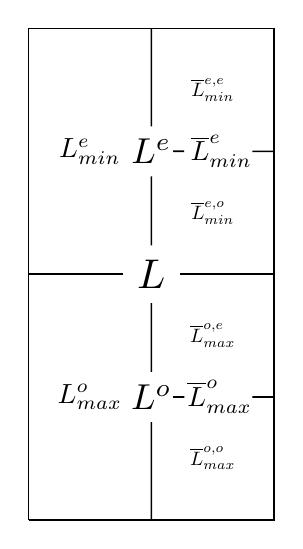
\begin{tikzpicture}[scale = .26]
		\node (L) at (0,0) [scale = 1.5]{$L$};
		\draw [semithick] (-6,0) -- (L) -- (6,0);
		\draw [semithick] (-6,-12) -- (6,-12) -- (6,12) -- (-6,12) -- (-6,-12);
		Statement
		\node (Le) at (0,6) [scale = 1.3] {$L^e$};
		\node (Lemax) at (-3,6) {$ {L}^e_{min}$};
		\node (-Lemax) at (3,6) {$\; \overline{L}^e_{min}$\!\!};
		\node at (3,3) [scale = .7] {$\overline{L}^{e,o}_{min}$};
		\node at (3,9) [scale = .7] {$\overline{L}^{e,e}_{min}$};
		
		\draw [semithick] (L) -- (Le) -- (0,12);
		\draw [semithick] (6,6) -- (-Lemax) -- (Le);
		
		\node (Lo) at (0,-6) [scale = 1.3] {$L^o$};
		\node (Lomin) at (-3,-6) {$ {L}^o_{max}$};
		\node (-Lomin) at (3,-6) {$\, \overline{L}^o_{max}$\!\!};
		\node at (3,-3) [scale = .7] {$\overline{L}^{o,e}_{max}$};
		\node at (3,-9) [scale = .7] {$\overline{L}^{o,o}_{max}$};
		
		\draw [semithick] (L) -- (Lo) -- (0,-12);
		\draw [semithick] (6,-6) -- (-Lomin) -- (Lo);
		\end{tikzpicture}
	\end{center}
\end{minipage}
\begin{minipage}{.8\textwidth}
	$L = \{x.U^- \tensor U^+\ | \ U \in \P_q(n),\ x \in \overline{U}\}$. \\
	\begin{tab}
		$L^{e} = \{x.U^- \tensor U^+ \in L\ | \ \ind_{x.U}(x) \text{ even}\}$. 
		\begin{tab}
			$L_{min}^{e} = \{x.U^- \tensor U^+ \in L^e\ | \ x < u_1 \}$.\par
			$\overline{L}_{min}^{e} = L^{e} \setminus L_{min}^{e}$.
			\begin{tab}
				$\overline{L}_{min}^{e,e} = \{ x.U^- \tensor U^+ \in \overline{L}_{min}^{e}\ | \ \ind_{x.U}(l_{U,x}) \text{ even} \}$.\par
				$\overline{L}_{min}^{e,o} = \{ x.U^- \tensor U^+ \in \overline{L}_{min}^{e}\ | \ \ind_{x.U}(l_{U,x}) \text{ odd} \}.$ \\
			\end{tab}
		\end{tab}
		$L^{o} = \{x.U^- \tensor U^+\ | \ \ind_{x.U}(x) \text{ odd}\}$.\par 
		\begin{tab}
			$L_{max}^{o} = \{x.U^- \tensor U^+ \in L^o\ | \ u_q < x \}$.\par
			$\overline{L}_{max}^{o} = L^{o}\setminus L_{max}^{o}$.
			\begin{tab}
				$\overline{L}_{max}^{o,e} = \{ x.U^- \tensor U^+ \in \overline{L}_{max}^{o}\ | \ \ind_{x.U}(r_{U,x}) \text{ even} \}$.\par 
				$\overline{L}_{max}^{o,o} = \{ x.U^- \tensor U^+ \in \overline{L}_{max}^{o}\ | \ \ind_{x.U}(r_{U,x}) \text{ odd} \}$.
			\end{tab}
		\end{tab}
	\end{tab}
\end{minipage}

\begin{minipage}{.3\textwidth}
	\begin{center}
		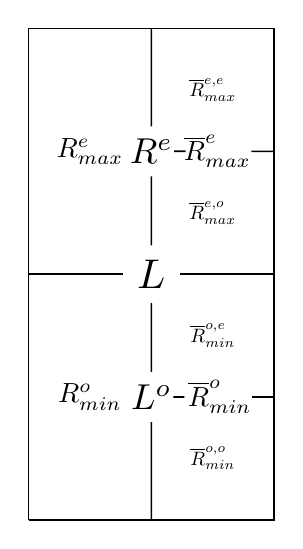
\begin{tikzpicture}[scale = .26]
		\node (L) at (0,0) [scale = 1.5]{$L$};
		\draw [semithick] (-6,0) -- (L) -- (6,0);
		\draw [semithick] (-6,-12) -- (6,-12) -- (6,12) -- (-6,12) -- (-6,-12);
		
		\node (Le) at (0,6) [scale = 1.3] {$R^e$};
		\node (Lemax) at (-3,6) {$ {R}^e_{max}$};
		\node (-Lemax) at (3,6) {$\overline{R}^e_{max}$\!\!};
		\node at (3,3) [scale = .7] {$\overline{R}^{e,o}_{max}$};
		\node at (3,9) [scale = .7] {$\overline{R}^{e,e}_{max}$};
		
		\draw [semithick] (L) -- (Le) -- (0,12);
		\draw [semithick] (6,6) -- (-Lemax) -- (Le);
		
		\node (Lo) at (0,-6) [scale = 1.3] {$L^o$};
		\node (Lomin) at (-3,-6) {$ {R}^o_{min}$};
		\node (-Lomin) at (3,-6) {\,$\overline{R}^o_{min}$\!\!};
		\node at (3,-3) [scale = .7] {$\overline{R}^{o,e}_{min}$};
		\node at (3,-9) [scale = .7] {$\overline{R}^{o,o}_{min}$};
		
		\draw [semithick] (L) -- (Lo) -- (0,-12);
		\draw [semithick] (6,-6) -- (-Lomin) -- (Lo);
		\end{tikzpicture}
	\end{center}
\end{minipage}
\begin{minipage}{.8\textwidth}
	$R = \{U^-\tensor x.U^+\ | \ U \in \P_q(n),\ x \in \overline{U}\}$.\\
	\begin{tab}
		$R^{e} = \{U^-\tensor x.U^+ \in R\ | \ \ind_{x.U}(x) \text{ even}\}$.\par
		\begin{tab}
			$R_{max}^{e} = \{U^- \tensor x.U^+ \in R^e\ | \ u_q < x \}$.\par 
			$\overline{R}_{max}^{e} = R^{e} \setminus R_{max}^{e}$.
			\begin{tab}
				$\overline{R}_{max}^{e,e} = \{ U^- \tensor x.U^+ \in \overline{R}_{max}^{e}\ | \ \ind_{x.U}(r_{U,x}) \text{ even} \}$.\par 
				$\overline{R}_{max}^{e,o} = \{ U^- \tensor x.U^+ \in \overline{R}_{max}^{e}\ | \ \ind_{x.U}(r_{U,x}) \text{ odd} \}$.\\
			\end{tab}
		\end{tab}
		$R^{o} = \{U^- \tensor x.U^+ \in R\ | \ \ind_{x.U}(x) \text{ odd}\}$.\par 
		\begin{tab}
			$R_{min}^{o} = \{U^- \tensor x.U^+ \in R^o \ | \  x < u_1 \}$.\par 
			$\overline{R}_{min}^{o} = R^{o} \setminus R_{min}^{o}$.
			\begin{tab}
				$\overline{R}_{min}^{o,e} = \{ U^- \tensor x.U^+ \in \overline{R}_{min}^{o}\ | \ \ind_{x.U}(l_{U,x}) \text{ even} \}$.\par 
				$\overline{R}_{min}^{o,o} = \{ U^- \tensor x.U^+ \in \overline{R}_{min}^{o}\ | \ \ind_{x.U}(l_{U,x}) \text{ odd} \}$.
			\end{tab}
		\end{tab}
	\end{tab}
\end{minipage} \\ \\
We claim the following four identities: 
\begin{equation}\label{lemma4: existence: eq2}
\overline{R}_{min}^{o,o} = \overline{L}_{max}^{o,o}\ , \qquad \overline{R}_{min}^{o,e} = \overline{R}_{max}^{e,o}\ , \qquad 
\overline{L}_{min}^{e,o} = \overline{L}_{max}^{o,e}\ , \qquad \overline{L}_{min}^{e,e} = \overline{R}_{max}^{e,e}.
\end{equation}
We show only the proof of the first one. The other three are proven analogously.
\begin{alignat*}{2}
&\boxed{U^-\tensor x.U^+ \in \overline{R}_{min}^{o,o}}\ &\Longrightarrow\ &\boxed{U^-\tensor x.U^+ =\, l_{U,x}.V_U(x)^-\tensor V_{U,x}^+ \in \overline{L}_{max}^{o,o} \ \ } \\ 
&\boxed{x.U^-\tensor U^+ \in \overline{L}_{max}^{o,o}}\ &\Longrightarrow\ &\boxed{x.U^-\tensor U^+ =\, W_U(x)^-\tensor r_{U,x}.W_{U,x}^+ \in \overline{R}_{min}^{o,o} \! }
\end{alignat*}
The identities in (\ref{lemma4: existence: eq2}) imply 
\begin{equation} \label{lemma4: existence: eq3} 
\sum_{\overline{L}_{max}^{o}} d_{x.U^-} \tensor d_{U^+}\ \ +\ \ 
\sum_{\overline{R}_{max}^{e}} d_{U^-} \tensor d_{x.U^+}\ \ +\ \ 
\sum_{\overline{L}_{min}^{e}} d_{x.U^-} \tensor d_{U^+}\ \ +\ \ 
\sum_{\overline{R}_{min}^{o}} d_{U^-} \tensor d_{x.U^+} = 0.
\end{equation}
Let us now consider the right hand side of (\ref{lemma4: existence: eq1})
\begin{equation*}
\sum_{U\in\P_{q+1}(n)} d_{U^-} \tensor d_{U^+} +\, d_{U^+} \tensor d_{U^-.}
\end{equation*}
Notice it is equal to
\begin{align*}
&\, \sum_{\substack{U \in \P_{q+1}(n) \\ \ind_U(u_{q+1}) \text{ odd}}} d_{u_{q+1}.(U \smallsetminus u_{q+1})^-} \tensor d_{(U \smallsetminus u_{q+1})^+}\ \ + 
\sum_{\substack{U \in \P_{q+1}(n) \\ \ind_U(u_{q+1}) \text{ even}}} d_{(U\smallsetminus u_{q+1})^-} \tensor d_{u_{q+1}.(U \smallsetminus u_{q+1})^+}\ \ + \\
&\ \,\sum_{\substack{U \in \P_{q+1}(n) \\ \ind_U(u_1) \text{ even}}} d_{u_1.(U\smallsetminus u_1)^-} \tensor d_{(U\smallsetminus u_1)^+}\ \ +
\sum_{\substack{U \in \P_{q+1}(n) \\ \ind_U(u_1) \text{ odd}}} d_{(U \smallsetminus u_1)^-} \tensor d_{u_1.(U\smallsetminus u_1)^+.}
\end{align*}
This expression, in turn, equals
\begin{equation*} 
\sum_{{L}_{max}^{o}} d_{x.U^-} \tensor d_{U^+}\ \ +\ \ 
\sum_{{R}_{max}^{e}} d_{U^-} \tensor d_{x.U^+}\ \ +\ \ 
\sum_{{L}_{min}^{e}} d_{x.U^-} \tensor d_{U^+}\ \ +\ \ 
\sum_{{R}_{min}^{0}} d_{U^-} \tensor d_{x.U^+.}
\end{equation*}
Thanks to (\ref{lemma4: existence: eq3}), the above expression equals
\begin{equation*}
\sum_{L} d_{x.U^-} \tensor d_{U^+}\ +\ \ 
\sum_{R} d_{U^-} \tensor d_{x.U^+,}
\end{equation*}
the left hand side of (\ref{lemma4: existence: eq1}).

The proof of Proposition \ref{proposition: chain map}, the chain map property, now follows directly from Lemma \ref{lemma3: existence} and Lemma \ref{lemma4: existence}.
	
\section{Secondary operations} \label{s:outlook}

%The speed gained with the proposed algorithm is key for the applications of Steenrod squares in topological data analysis.

Lifting relations from the (co)homology level to the (co)chain level is often a source of further structure.
For example, cup-$i$ products provide an effective construction of coboundaries coherently enforcing the commutativity relation of the cup product in cohomology.

It is natural then to wonder about what relations are satisfied by Steenrod squares themselves.
There are two notable relations to consider.
The first one, known as the \textit{Cartan relation}, expresses the interaction between these operations and the cup product:
\begin{equation*}
Sq^k \big( [\alpha] [\beta] \big) = \sum_{i+j=k} Sq^i \big([\alpha]\big)\, Sq^j \big([\beta]\big),
\end{equation*}
whereas the second, the \textit{Adem relation} \cite{adem52relations}, expresses dependencies appearing through iteration:
\begin{equation} \label{equation: adem relations}
Sq^i Sq^j = \sum_{k=0}^{\lfloor i/2 \rfloor} {j-k-1 \choose i-2k} Sq^{i+j-k} Sq^k,
\end{equation}
where $\lfloor- \rfloor$ denotes the integer part function and the binomial coefficient is reduced mod $2$.

To tap into the secondary structure associated with these relations, one needs to provide effective proofs for them, that is to say, construct explicit cochains enforcing them when passing to cohomology.
Such effective proofs were recently given respectively in \cite{medina2020cartan} and \cite{medina2020adem}, and we expect the additional structure they unlock will also play an important role in computational topology.
	\bibliographystyle{ieeetr}
	\bibliography{bibliography}
\end{document}
